%
% $File: report.tex
% $Date: Sun Dec 01 21:22:10 2013 +0800
%

\documentclass{article}
\usepackage{fontspec}
\usepackage{zhspacing,url,amsmath,amssymb,verbatim}
\usepackage{pdfpages}
\zhspacing
\usepackage{listings}
\usepackage[hyperfootnotes=false,colorlinks,linkcolor=blue,anchorcolor=blue,citecolor=blue]{hyperref}
\usepackage[backend=biber]{biblatex}
\usepackage{graphicx}
\usepackage{minted}
\usepackage{subfigure}
\usepackage{indentfirst}
\usepackage{cases}
\usepackage{environ}
\usepackage{array}
\usepackage[top=1in, bottom=1in, left=1.25in, right=1.25in]{geometry}
\usepackage{caption}
%\usepackage{tikz}
%\usepackage{dot2texi}

% $File: mint-defs.tex
% $Date: Sun Nov 17 23:37:24 2013 +0800
% $Author: Xinyu Zhou <zxytim@gmail.com>

\newcommand{\inputmintedConfigured}[3][]{\inputminted[fontsize=\footnotesize,
	label=#3,linenos,frame=lines,framesep=0.8em,tabsize=4,#1]{#2}{#3}}

\newcommand{\txtsrc}[2][]{\inputmintedConfigured[#1]{text}{#2}}
\newcommand{\txtsrcpart}[4][]{\txtsrc[firstline=#3,firstnumber=#3,lastline=#4,#1]{#2}}

\newcommand{\cppsrc}[2][]{\inputmintedConfigured[#1]{cpp}{#2}}
\newcommand{\cppsrcpart}[4][]{\cppsrc[firstline=#3,firstnumber=#3,lastline=#4,#1]{#2}}

\newcommand{\javasrc}[2][]{\inputmintedConfigured[#1]{java}{#2}}
\newcommand{\javasrcpart}[4][]{\javasrc[firstline=#3,firstnumber=#3,lastline=#4,#1]{#2}}

\newcommand{\matlabsrc}[2][]{\inputmintedConfigured[#1]{matlab}{#2}}
\newcommand{\matlabsrcpart}[4][]{\matlabsrc[firstline=#3,firstnumber=#3,lastline=#4,#1]{#2}}

\newcommand{\pysrc}[2][]{\inputmintedConfigured[#1]{matlab}{#2}}
\newcommand{\pysrcpart}[4][]{\matlabsrc[firstline=#3,firstnumber=#3,lastline=#4,#1]{#2}}

%\usepackage[T1]{fontenc}
\usepackage{lmodern}
\usepackage{amssymb,amsmath}
\usepackage{ifxetex,ifluatex}
\usepackage{fixltx2e} % provides \textsubscript
% use upquote if available, for straight quotes in verbatim environments
\IfFileExists{upquote.sty}{\usepackage{upquote}}{}
\ifnum 0\ifxetex 1\fi\ifluatex 1\fi=0 % if pdftex
  \usepackage[utf8]{inputenc}
\else % if luatex or xelatex
  \usepackage{fontspec}
  % commented by Xinyu Zhou
  \ifxetex
    \usepackage{xltxtra,xunicode}
  \fi
  \defaultfontfeatures{Mapping=tex-text,Scale=MatchLowercase}
  \newcommand{\euro}{€}
\fi
% use microtype if available
\IfFileExists{microtype.sty}{\usepackage{microtype}}{}
\usepackage{color}
\usepackage{fancyvrb}
\newcommand{\VerbBar}{|}
\DefineShortVerb[commandchars=\\\{\}]{\|}
\DefineVerbatimEnvironment{Highlighting}{Verbatim}{commandchars=\\\{\}}
% Add ',fontsize=\small' for more characters per line
\newenvironment{Shaded}{}{}
\newcommand{\KeywordTok}[1]{\textcolor[rgb]{0.00,0.44,0.13}{\textbf{{#1}}}}
\newcommand{\DataTypeTok}[1]{\textcolor[rgb]{0.56,0.13,0.00}{{#1}}}
\newcommand{\DecValTok}[1]{\textcolor[rgb]{0.25,0.63,0.44}{{#1}}}
\newcommand{\BaseNTok}[1]{\textcolor[rgb]{0.25,0.63,0.44}{{#1}}}
\newcommand{\FloatTok}[1]{\textcolor[rgb]{0.25,0.63,0.44}{{#1}}}
\newcommand{\CharTok}[1]{\textcolor[rgb]{0.25,0.44,0.63}{{#1}}}
\newcommand{\StringTok}[1]{\textcolor[rgb]{0.25,0.44,0.63}{{#1}}}
\newcommand{\CommentTok}[1]{\textcolor[rgb]{0.38,0.63,0.69}{\textit{{#1}}}}
\newcommand{\OtherTok}[1]{\textcolor[rgb]{0.00,0.44,0.13}{{#1}}}
\newcommand{\AlertTok}[1]{\textcolor[rgb]{1.00,0.00,0.00}{\textbf{{#1}}}}
\newcommand{\FunctionTok}[1]{\textcolor[rgb]{0.02,0.16,0.49}{{#1}}}
\newcommand{\RegionMarkerTok}[1]{{#1}}
\newcommand{\ErrorTok}[1]{\textcolor[rgb]{1.00,0.00,0.00}{\textbf{{#1}}}}
\newcommand{\NormalTok}[1]{{#1}}
% \ifxetex
%   \usepackage[setpagesize=false, % page size defined by xetex
%               unicode=false, % unicode breaks when used with xetex
%               xetex]{hyperref}
% \else
%   \usepackage[unicode=true]{hyperref}
% \fi
\hypersetup{breaklinks=true,
            bookmarks=true,
            pdfauthor={},
            pdftitle={},
            colorlinks=true,
            urlcolor=blue,
            %linkcolor=magenta,
            pdfborder={0 0 0}}
%\urlstyle{same}  % don't use monospace font for urls
\setlength{\parindent}{0pt}
\setlength{\parskip}{6pt plus 2pt minus 1pt}
\setlength{\emergencystretch}{3em}  % prevent overfull lines
%\setcounter{secnumdepth}{0}



\newcommand{\figref}[1]{\hyperref[fig:#1]{Figure\ref*{fig:#1}}}
\newcommand{\tableref}[1]{\hyperref[table:#1]{Table\ref*{table:#1}}}
\newcommand{\centerize}[1]{\begin{center} #1 \end{center}}

\newcommand{\cmd}[1]{{\it #1}}
\newcommand{\ccmd}[1]{\centerize{\cmd{#1}}}

\title{Digital Signal Processing: Speaker Recognition \\ Midterm Report}
\author{Xinyu Zhou, Yuxin Wu, and Tiezheng Li\\ Tsinghua University}
\date{}

\bibliography{refs.bib}
\begin{document}

\fontsize{11pt}{1.4em}
\setlength{\baselineskip}{1.6em}
\maketitle

\section{Task}
	Build a speaker recognition system

\section{Dataset}
\label{sec:data}
  In the filed of speech/speaker recognition, there are some research oriented
  corpus, but most of them are expensive. \cite{database} gives a detailed list on the
  popular speech corpus for speech/speaker recognition. In this system,
  we mainly use the speech corpus provided by our teacher Xu.

	The dataset provided comprised of 102 speaker, in which 60 are
	females and the rest are males.
    The dataset contains three different speaking style: Spontaneous,
	Reading and Whisper. Some simple statistics are as follows:
	\begin{table}[!ht]
		\centering
		\begin{tabular}{|c|c|c|c|}
			\shline
			& Spontaneous & Reading & Whisper \\\shline
			Average Duration & 202s & 205s & 221s \\\hline
			Female Average Duration & 205s & 202s & 217s \\\hline
			Male Average Duration & 200s & 203s & 223s \\\shline
		\end{tabular}
	\end{table}



\section{Approach}
The task of speaker recognition can be considered as a task of classification. Thus a number of machine learning techniques
can be applied to this task. In general, this task should cover the following three topics:

\begin{enumerate}
  \item Feature Extraction: process the voice signal and extract acoustic features that
	  could describe the acoustic characteristics of speakers, which can be correlated
	  in some extend to model latter used.

  \item Acoustic Model: provide the functionality of registration as well as identification or verification.

  \item Evaluation: Evaluate our approach using datasets with appropriate metrics.
\end{enumerate}

\subsection{Feature Extraction}
The task of speaker recognition is highly correlated to the task of speech recognition.
In the field of speech recognition, Complex Cepstrum \cite{cepstrum} is
considered to be a concise description to the original acoustic signal.
In particular, Mel-frequency Cepstral Coefficients (MFCC), is a state-of-the-art standard feature
widely used in Automatic Speech Recognition (ASR) system.
The general procedure for calculating MFCC is as follows:
\begin{figure}[H]
  \centering
  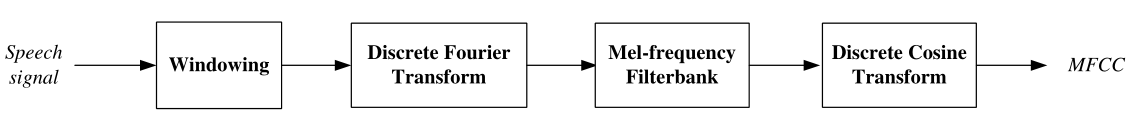
\includegraphics[width=\textwidth]{res/MFCC.png}
\end{figure}

As for speaker recognition, several different features are suggested and compared
by researchers \cite{evaluation}. Cepstrum still proves to be a robust and effective
feature in this task. Therefore, a bunch of cepstral features, including MFCC,
LPCC (Linear Prediction Cepstrum Coefficients), are commonly used
in speaker recognition system.\cite{feature}

We plan to implement common cepstral features used by researchers, and use a
combination of some of them, according to the further observation and test on how
much they contribute to the task.

\subsection{Model}
According to works in years, Gaussian Mixture Model (GMM)
has been a common approach to acoustic modeling.\cite{GMM}
GMM can be used to acquire an acoustic model $P(\mathbf{O} | \mathbf{W}) $,
which gives the probability of a given observation
$\mathbf{O}$ under certain word $\mathbf{W}$. By using GMM, this
conditional probability can be well estimated by modeling the distribution as
a sum of several normal distribution.

In addition to that, Hidden Markov Model (HMM) is a main-stream approach in ASR system,
since it can describe sequential relation of observations.\cite{SLP}
We have noticed a few research-oriented open-source speech recognition
tool building on HMM, such as HTK\cite{htk}.
Such tools might be quite useful in buiding a speaker recognition system.

Recently, some common machine learning model are also applied to the task of speaker
recognition. \cite{svm} suggested a method of using SVM in speaker recognition.
Deep neural networks are also used in speech processing recently.\cite{deep}

HMM and GMM will probably be our first attempt, as they are already widely used and proven to be
efficient and effective.  We might also try to migrate our extracted feature to
some other available models.

\subsection{Evaluation}
\subsubsection{Dataset}
There are a number of well-known databses for speaker recognition system evaluation,
such as KING speaker verification\cite{king}. \cite{database} gives description on
several common databases. But most of these databases are not free of charge.
We intend to search for an freely available database,
otherwise we have to build some simple test cases by our own.
\subsubsection{Metrics}
As we intend to distinguish different speakers, the primary goal is overall
accuracy of the system we built. Furthermore, the performance may differ from
speaker to speaker, which may provide with additional feedback to our approach.
Thus we shall examine precision, recall and $F_1$ score for each speaker.



\section{Progress}
	During past weeks, we've built a proof-of-concept ASR system based on
	MFCC feature and GMM for modeling spearker with fine-tuned parameters.

	A brief performance summary:
	\begin{itemize}
		\item $10s\sim15s$ training corpus per person.
		\item $2s\sim5s$ test corpus per person.
		\item We adopted GMM with $32$ Gaussians.
		\item Accuracy on 5 speakers is about 93 percent
		\item Accuracy on 10 speakers is about 90 percent
	\end{itemize}

	It turns out that, our method worked well when the condition that the number of
	speakers is limited to 5 or less is met. But as we employed the new dataset
	which provided by teacher this week, which contains 102 speaker, comprised
	of 60 females and 42 males, in three speaking conditions: reading,
	spontaneous and whisper, the challenge we are facing is beyond our expectation.

	Although we fulfilled the plan we aforementioned in opening report, the overall
	performance is still unsatisfying.
	The main reason that MFCC + GMM approach suffers from new corpus is that,
	using solely MFCC limits the model we can use to generative models,
	which in turns brings computation inefficiency to feature extraction, model
	training and testing.



\section{Analysis}
	The result indicates the effectiveness of our method, but also shows the limitation.
	\begin{enumerate}
		\item The performance is not satisfying. \\
			Compare to the performance given in serval sources (books and papers),
			ours are not the best.  This may due to the corpus difference between
			test, and the result may not be comparable.
			But comparing to MFCC extractor provided by
			bob\cite{bob2012}, we get $5\%$ higher accuracy, which proved the
			effectiveness of our model.
		\item Long training utterance. \\
			30s utterance training data may not feasible in practical application.
		\item GMM is of low efficiency when classifying. \\
			Due to the modeling of each spkeaker using GMM with 32 mixtures,
			classification of a single speaker involves scoring over all
			enrolled speakers. The more speaker, the less efficiency.
	\end{enumerate}


\section{Next Step}

Our proposed way to workaround the situation mentioned in previous chapter is using
supervector-based approaches. This is advantageous since it map a speech to a single
vector, which makes it easy to utilizes discrimitive models that are more powerful
in classification task, such as SVM. Further more,
we plan to conduct extensive investigation on \textbf{Joint Factor Analysis(JFA)}
, which is a much promising method to our best knowledge extent.


\printbibliography

\end{document}

